\section{Análisis económico y evaluación financiera del escenario anual}
\label{sec:analisis-anual}

\subsection{Cómo se relacionan los cálculos de la proyección}

La cantidad de gimnasios activos depende de las contrataciones y cancelaciones.
Sus planes determinan cuánto se cobraría, mientras que la instalación, el uso
y el soporte generan costos. En esta sección se relacionan esos cálculos para
estimar el primer año del servicio. Las tablas y gráficas son de elaboración
propia a partir del escenario financiero preliminar.

Se denomina ingreso mensual recurrente, o MRR, a las mensualidades previstas de
los clientes activos. Un cliente Starter aporta CRC 15\,000 y cada Pro Gym
aporta CRC 25\,000. Si \(N\) representa la cantidad de gimnasios y uno de ellos
mantiene Starter, el ingreso mensual se calcula así:
\[
 I(N)=15\,000+25\,000(N-1).
\]
El precio promedio cambia según los planes contratados: CRC 23\,000 con cinco clientes y
CRC 24\,285,71 con catorce. El promedio anual de CRC 23\,965,52 corresponde a
CRC 2\,780\,000 entre 116 meses-cliente, no al precio de un plan adicional.
Un mes-cliente representa un gimnasio activo durante un mes.

\subsection{Cartera y presupuesto de ingresos}

\begin{longtable}{lrrrr}
\caption{Cartera e ingresos mensuales proyectados}\\
\toprule
Mes & Altas & Bajas & Activos & Ingreso CRC \\
\midrule
\endfirsthead
\toprule
Mes & Altas & Bajas & Activos & Ingreso CRC \\
\midrule
\endhead
1 & 5 & 0 & 5 & 115\,000,00 \\
2 & 1 & 0 & 6 & 140\,000,00 \\
3 & 1 & 0 & 7 & 165\,000,00 \\
4 & 1 & 0 & 8 & 190\,000,00 \\
5 & 1 & 0 & 9 & 215\,000,00 \\
6 & 1 & 1 & 9 & 215\,000,00 \\
7 & 1 & 0 & 10 & 240\,000,00 \\
8 & 1 & 0 & 11 & 265\,000,00 \\
9 & 1 & 0 & 12 & 290\,000,00 \\
10 & 1 & 1 & 12 & 290\,000,00 \\
11 & 1 & 0 & 13 & 315\,000,00 \\
12 & 1 & 0 & 14 & 340\,000,00 \\
\bottomrule
\end{longtable}
{\small\textit{Nota}. Elaboración propia a partir del escenario financiero preliminar. Se cobra el mes completo desde el alta y se mantiene un cliente Starter.}


La tabla comienza con cinco altas y suma una en cada mes posterior.
Las cancelaciones de los meses 6 y 10 hacen que la cantidad permanezca en nueve
y doce gimnasios, respectivamente, aunque se incorpora una nueva cuenta. El
modelo supone que las bajas no eliminan al único Starter, que las mensualidades
se cobran completas desde el alta y que no existen descuentos, impagos o ventas
de planes Premium y Enterprise. Si estas condiciones cambian, la proyección
debe ajustarse.

\begin{figure}[htbp]
\centering
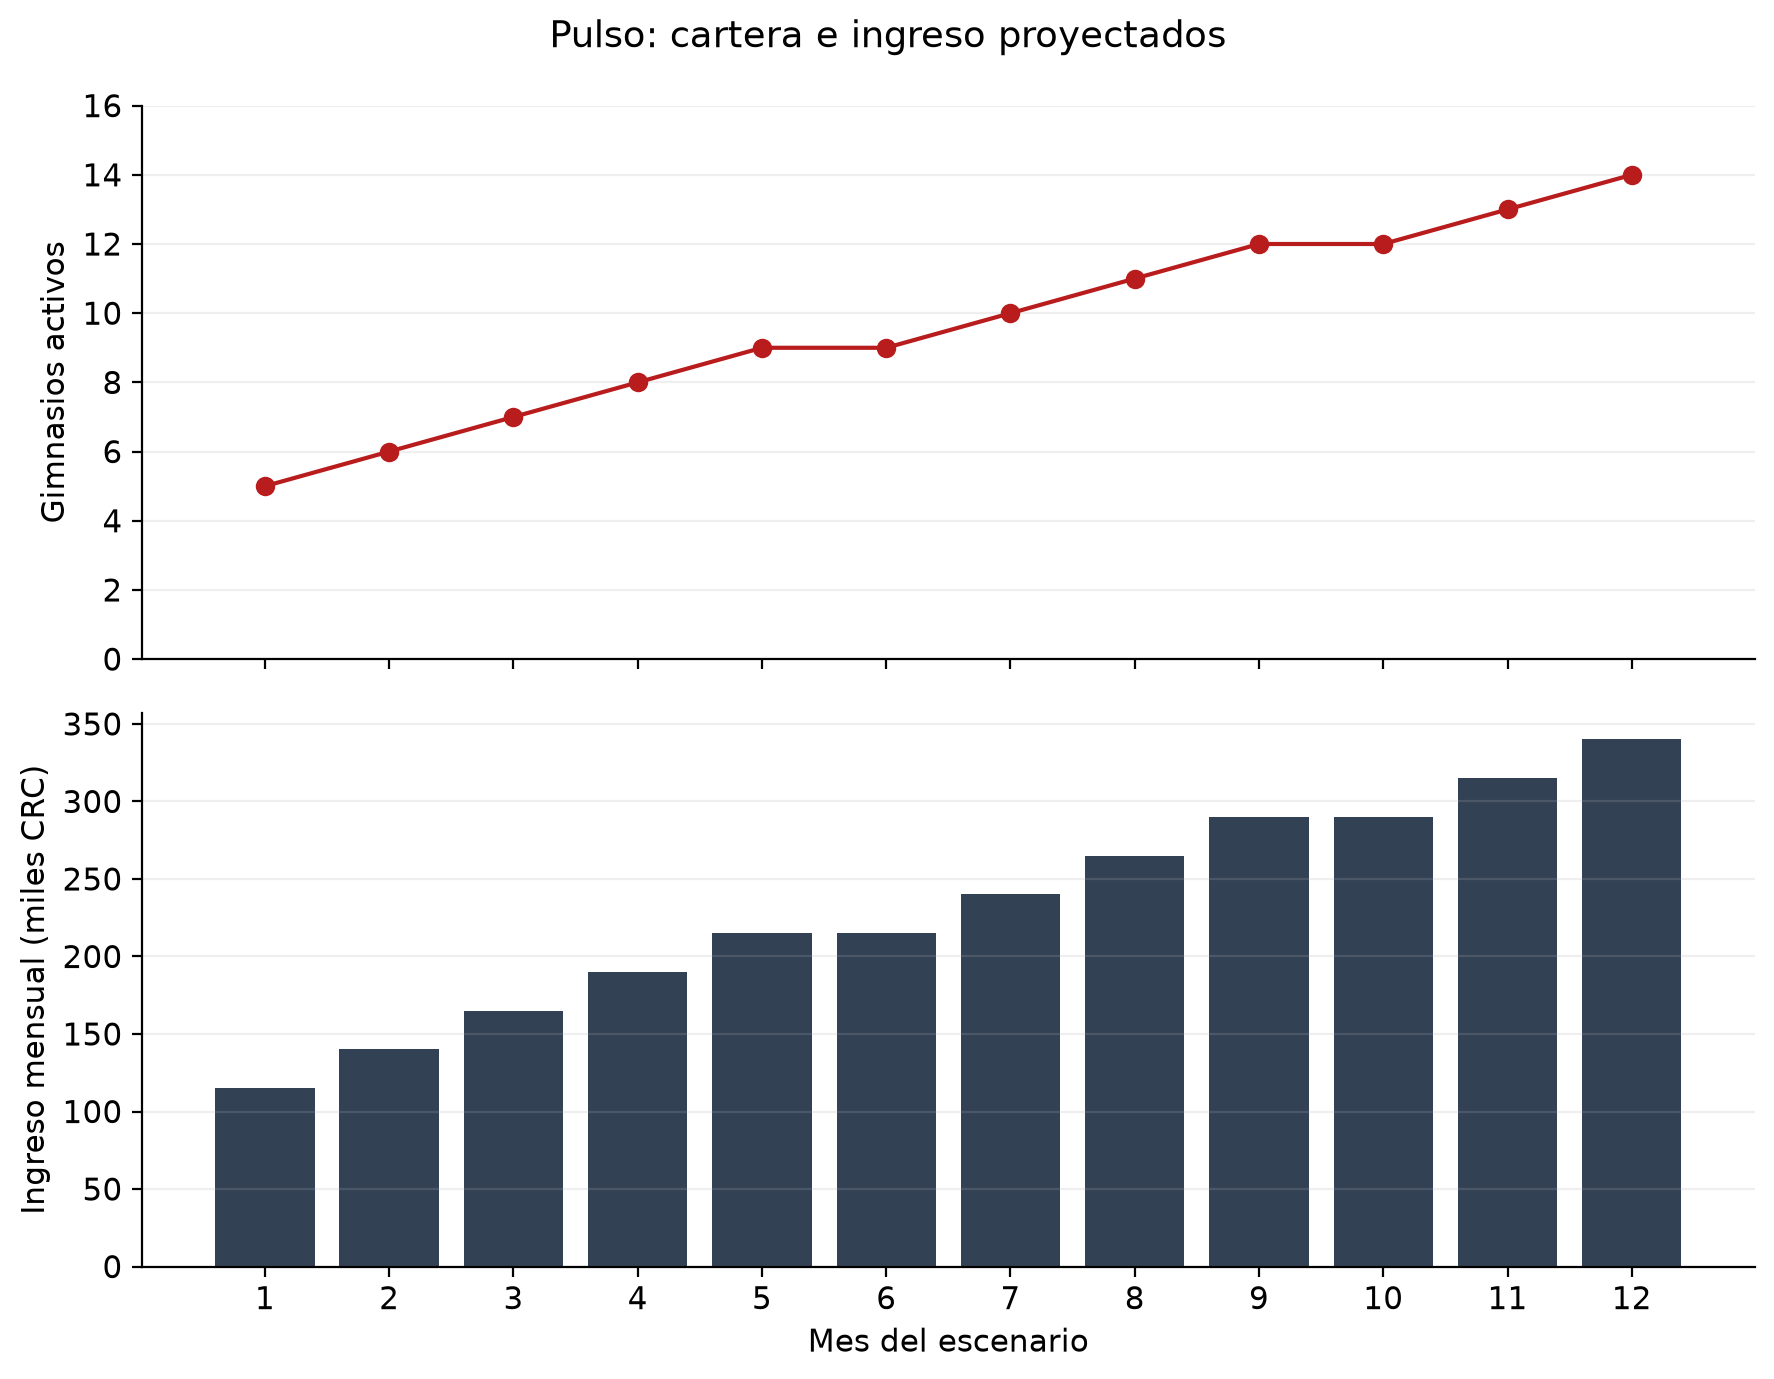
\includegraphics[width=.94\textwidth]{imagenes/excel_cartera_ingresos.png}
\caption{Evolución proyectada de clientes e ingreso mensual}
\label{fig:cartera-excel}
\caption*{\textit{Nota}. Elaboración propia a partir del escenario financiero preliminar del año 1.}
\end{figure}

En la Figura~\ref{fig:cartera-excel}, los tramos sin aumento corresponden a
meses con una contratación y una cancelación. Los catorce clientes se alcanzan
al cierre; cada gimnasio aporta ingresos desde el mes en que entra.

\subsection{Egresos, trabajo aportado y puesta en marcha}

La base mensual de CRC 114\,247,54 suma infraestructura por CRC 58\,125,
viáticos por CRC 12\,000, publicidad por CRC 5\,000, correo y diseño por
CRC 6\,000 y trabajo de mantenimiento y captación por CRC 33\,122,54.
En el primer mes los gastos fijos económicos suben a CRC 191\,931,36 por
mayores viáticos y horas comerciales. El costo de soporte se modela con
media hora mensual por gimnasio; la instalación agrega ocho horas por alta.

Los costos variables del primer mes ascienden a CRC 89\,964,55 e incluyen
las cinco incorporaciones. Los egresos económicos anuales sin el desarrollo
inicial suman CRC 1\,985\,220,37; al agregar CRC 198\,735,27 de desarrollo,
el costo económico total del escenario es CRC 2\,183\,955,64. Estos importes
incluyen trabajo sin desembolso, por lo que no coinciden con los pagos externos.

\begin{figure}[htbp]
\centering
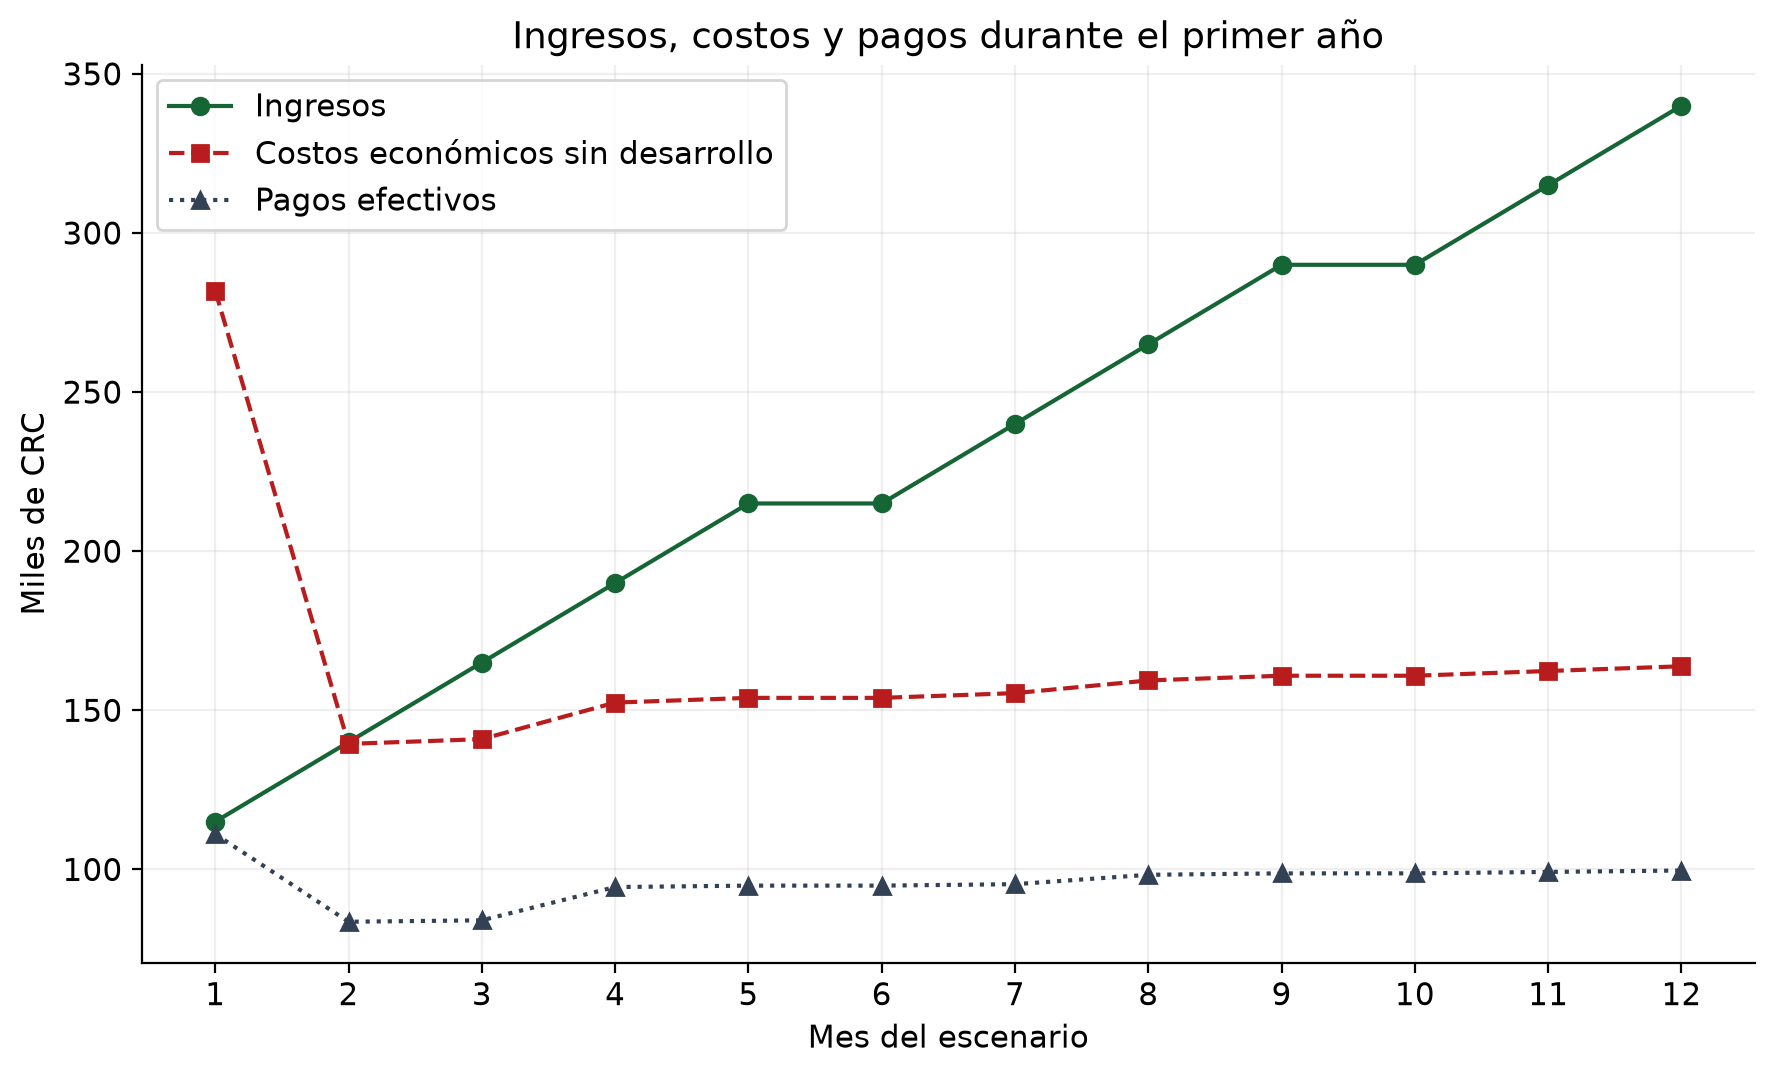
\includegraphics[width=\textwidth]{imagenes/excel_ingresos_egresos.png}
\caption{Comparación de ingresos, costos económicos y pagos efectivos}
\label{fig:egresos-excel}
\caption*{\textit{Nota}. Elaboración propia a partir del escenario financiero preliminar. La curva de costos excluye el desarrollo inicial.}
\end{figure}

La Figura~\ref{fig:egresos-excel} muestra que el mes 1 cuesta más por la
preparación inicial. Después, los costos crecen con los clientes y el uso.
La diferencia entre costos y pagos es el valor del trabajo que aporta el
equipo sin cobrarlo.

\subsection{Equilibrio operativo y margen de contribución}

El margen de contribución es lo que queda del precio después del costo variable
para cubrir costos fijos. Para la combinación inicial se calcula un precio
medio de CRC 23\,000 y un costo variable de CRC 1\,431,64, con una contribución
de CRC 21\,568,36 por gimnasio. Este promedio corresponde a cinco clientes
y debe revisarse cuando cambie la cantidad o la combinación de planes.

El cálculo del equilibrio da 5,2724 gimnasios cuando se mantiene un Starter
y se agregan Pro Gym, antes de los aumentos de infraestructura. Como los
clientes se cuentan en unidades completas, se comparan cinco y seis:
cinco dejan una pérdida de CRC 6\,405,73 y seis dejan CRC 17\,108,78 después
de cubrir la operación. El cálculo usa precios y costos que cambian con la
cantidad de clientes; por eso no coincide exactamente con dividir los costos
fijos entre el margen promedio anterior. Excluye instalación y desarrollo inicial.

\begin{figure}[htbp]
\centering
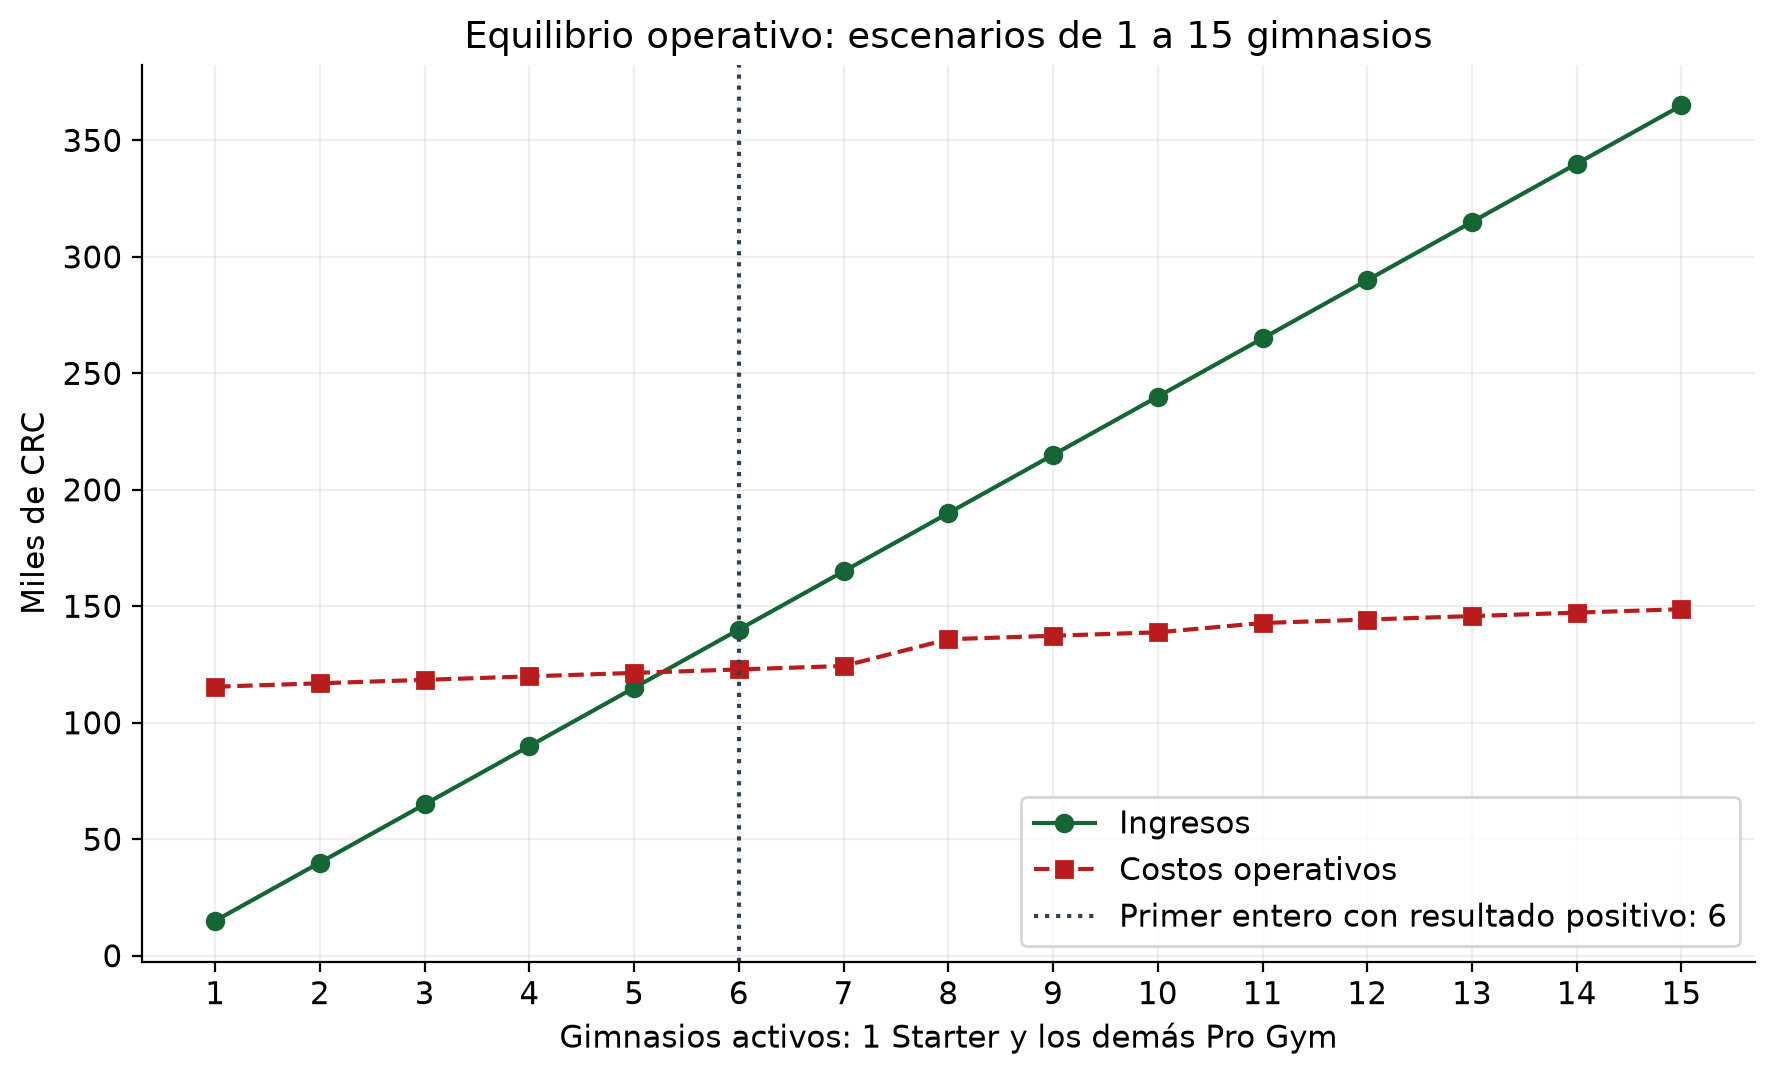
\includegraphics[width=\textwidth]{imagenes/excel_equilibrio_completo.png}
\caption{Sensibilidad del equilibrio a la cantidad de gimnasios activos}
\label{fig:equilibrio-completo}
\caption*{\textit{Nota}. Elaboración propia a partir del escenario financiero preliminar, de 1 a 15 gimnasios. Complementa el detalle de 4 a 8 presentado anteriormente.}
\end{figure}

En ocho y once gimnasios se observan cambios de costo asociados a la capacidad
de nube modelada. Por eso aumentar clientes no aumenta siempre el resultado en
la misma cantidad. Además, el mes 2 incluye una nueva instalación: sus ingresos
de CRC 140\,000 menos egresos económicos de CRC 139\,452,49 dejan solamente
CRC 547,51, aunque la tabla de operación estable muestra CRC 17\,108,78.
La diferencia se debe al costo de instalar la nueva cuenta en ese mes.

\subsection{Flujo de caja y necesidad de liquidez}

La caja es el dinero disponible para pagar. Las horas que aporta el equipo
tienen valor económico, pero no salen de la caja mientras no se paguen.
El aporte de CRC 40\,000 se suma al dinero inicial. Cada mes se calcula:
\[
 \mbox{Caja final}=\mbox{Caja anterior}+\mbox{aportes}+
 \mbox{cobros}-\mbox{pagos}.
\]

\begin{longtable}{lrrr}
\caption{Flujo mensual y resultado económico proyectados}\\
\toprule
Mes & Pagos CRC & Caja final CRC & Resultado CRC \\
\midrule
\endfirsthead
\toprule
Mes & Pagos CRC & Caja final CRC & Resultado CRC \\
\midrule
\endhead
1 & 111\,107,79 & 43\,892,21 & -365\,631,18 \\
2 & 83\,558,20 & 100\,334,01 & 547,51 \\
3 & 84\,008,61 & 181\,325,40 & 24\,062,02 \\
4 & 94\,459,02 & 276\,866,38 & 37\,576,53 \\
5 & 94\,909,43 & 396\,956,95 & 61\,091,04 \\
6 & 94\,909,43 & 517\,047,52 & 61\,091,04 \\
7 & 95\,359,84 & 661\,687,68 & 84\,605,55 \\
8 & 98\,310,25 & 828\,377,43 & 105\,620,06 \\
9 & 98\,760,66 & 1\,019\,616,77 & 129\,134,57 \\
10 & 98\,760,66 & 1\,210\,856,11 & 129\,134,57 \\
11 & 99\,211,07 & 1\,426\,645,04 & 152\,649,08 \\
12 & 99\,661,48 & 1\,666\,983,56 & 176\,163,59 \\
\bottomrule
\end{longtable}
{\small\textit{Nota}. Elaboración propia a partir del escenario financiero preliminar. La caja incluye CRC 40 000 de aporte inicial. El resultado del mes 1 incluye todo el costo del desarrollo.}


Los pagos anuales suman CRC 1\,153\,016,44. Los ingresos de CRC 2\,780\,000 y
el aporte de CRC 40\,000 producen una caja final de CRC 1\,666\,983,56.
La reserva de CRC 40\,000 se conserva como monto inicial propuesto. Para saber
si alcanza hay que comparar las fechas de cobro y pago. Aunque el mes 1 deja
CRC 3\,892,21 después de pagar, podría haber gastos que venzan antes de recibir
las mensualidades. El total mensual no permite conocer esa necesidad diaria.

\begin{figure}[htbp]
\centering
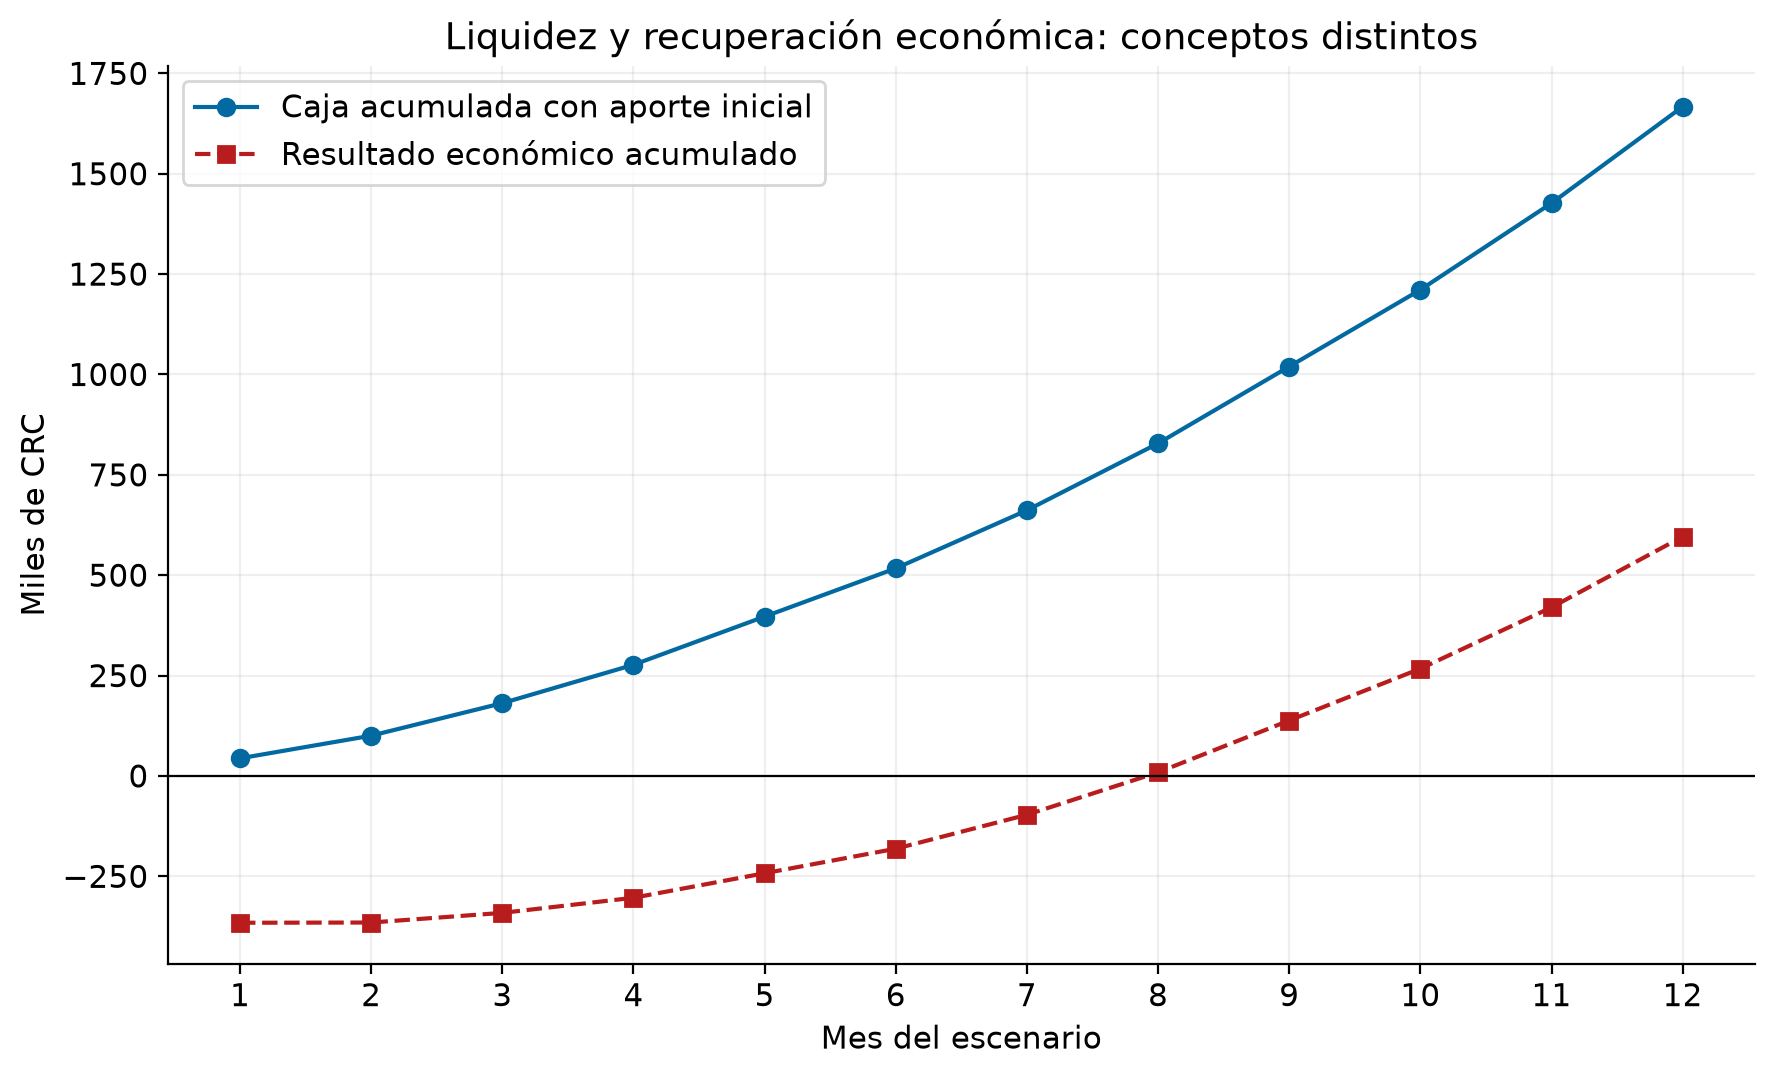
\includegraphics[width=\textwidth]{imagenes/excel_caja_resultado.png}
\caption{Caja acumulada y recuperación económica del trabajo invertido}
\label{fig:caja-recuperacion}
\caption*{\textit{Nota}. Elaboración propia a partir del escenario financiero preliminar. El resultado acumulado resta los costos económicos e incluye todo el desarrollo en el mes 1.}
\end{figure}

En la Figura~\ref{fig:caja-recuperacion} puede haber dinero disponible mientras
aún falta recuperar el valor del trabajo invertido. Al contar ese trabajo, el
resultado acumulado sigue negativo hasta el mes 7: pasa de
CRC $-96\,657,51$ a CRC 8\,962,55 en el mes 8. Esa sería la recuperación
simple si se cumplen los supuestos. El cálculo no ajusta el valor del dinero
por el paso del tiempo.

\subsection{Estado de resultados, balance e indicadores}

\Needspace{10\baselineskip}
\begin{longtable}{lrr}
\caption{Estado de resultados anual proyectado}\\
\toprule
Concepto & CRC & \% de ingresos \\
\midrule
\endfirsthead
\toprule
Concepto & CRC & \% de ingresos \\
\midrule
\endhead
Ingresos & 2\,780\,000,00 & 100,00 \\
Costos directos & 536\,566,02 & 19,30 \\
Utilidad bruta & 2\,243\,433,98 & 80,70 \\
Gastos fijos & 1\,448\,654,35 & 52,11 \\
Resultado antes del desarrollo & 794\,779,63 & 28,59 \\
Desarrollo del año & 198\,735,27 & 7,15 \\
Resultado antes de impuestos & 596\,044,36 & 21,44 \\
\bottomrule
\end{longtable}
{\small\textit{Nota}. Elaboración propia a partir del escenario financiero preliminar. Se presenta el resultado antes de impuestos porque falta confirmar las obligaciones del negocio.}


La utilidad bruta es lo que queda del ingreso después de los costos directos.
Al restar también los gastos fijos y el desarrollo se obtiene un
resultado antes de impuestos de CRC 596\,044,36, equivalente al 21,44\% de los
ingresos. Es decir, quedarían CRC 21,44 por cada CRC 100 de ingreso antes de
impuestos. Esto permite comparar escenarios, pero todavía habría que revisar
los pagos pendientes y las reservas antes de repartir dinero.

El borrador del presupuesto consideró impuesto cero bajo un supuesto de
formalización MYPE. Ese beneficio no está confirmado para Pulso. Por eso el
informe presenta el resultado antes de impuestos. El monto final se calculará
cuando se conozcan las obligaciones que corresponden al negocio.

\Needspace{10\baselineskip}
\begin{longtable}{lr}
\caption{Balance económico proyectado al cierre}\\
\toprule
Cuenta & CRC \\
\midrule
\endfirsthead
\toprule
Cuenta & CRC \\
\midrule
\endhead
Efectivo y activos totales & 1\,666\,983,56 \\
Deuda financiera & 0,00 \\
Aportes de efectivo y trabajo & 1\,070\,939,20 \\
Resultado económico del escenario & 596\,044,36 \\
Patrimonio total & 1\,666\,983,56 \\
\bottomrule
\end{longtable}
{\small\textit{Nota}. Elaboración propia a partir del escenario financiero preliminar. El trabajo se aporta sin pago y sin registrarlo como deuda. El tratamiento contable definitivo se revisará al formalizar el negocio.}


El patrimonio modelado suma aportes de efectivo y trabajo por CRC 1\,070\,939,20
más resultado económico por CRC 596\,044,36. Del primer importe, CRC 40\,000
corresponden al aporte de caja y CRC 1\,030\,939,20 a trabajo valorado. Por tanto:
\[
 40\,000+1\,030\,939{,}20+596\,044{,}36=1\,666\,983{,}56.
\]
La igualdad explica el balance proyectado sin deuda. En este ejercicio, todo
el desarrollo se registra como gasto del año, en vez de repartir su valor
entre varios periodos. El registro contable definitivo se revisará al
formalizar el negocio.

\subsection{Financiamiento y efecto sobre la permanencia}

El escenario base combina aporte propio de efectivo, equipos disponibles y
trabajo sin pago. Reduce la presión de caja, pero depende de que el equipo
disponga de tiempo y recursos. La sostenibilidad debe comprobarse también
cuando el servicio necesite remunerar ese trabajo.

\begin{longtable}{p{3cm}p{4.8cm}p{6.2cm}}
\caption{Alternativas de financiamiento y efecto esperado}\\
\toprule Alternativa & Aporte y ventaja & Condición o efecto sobre permanencia \\
\midrule\endfirsthead
\toprule Alternativa & Aporte y ventaja & Condición o efecto sobre permanencia \\
\midrule\endhead
Recursos propios & CRC 40\,000 de efectivo y trabajo aportado en el escenario. & No agrega deuda; depende de disponibilidad real y de no retirar recursos esenciales. \\
Reinversión de cobros & Utilizar excedentes para continuidad, soporte y capacidad. & Depende de cobros reales y reserva; un saldo proyectado no autoriza gastos anticipados. \\
Crédito eventual & Podría cubrir desfases de caja o inversión adicional. & Sin oferta ni aprobación. Debe cotizarse plazo, interés, garantías y cuotas antes de modelarlo. \\
Capital o apoyo externo & Podría aportar recursos o acompañamiento. & Sin compromiso confirmado. Revisar condiciones, participación y responsabilidad antes de considerarlo disponible. \\
\bottomrule
\end{longtable}
{\small\textit{Nota}. Elaboración propia. Solo los recursos propios forman
parte del escenario financiero preliminar.}

La reserva se revisará según las fechas de pago y cobro y las cancelaciones.
El análisis se limita al margen, el flujo de caja, el equilibrio y la
recuperación simple. Para calcular valor actual neto o tasa interna de retorno
haría falta definir más años de operación, una tasa para comparar el valor del
dinero en el tiempo y el valor del negocio al final de ese periodo.

\subsection{Sensibilidad, controles y conclusión financiera}

Una reducción del 10\% en los ingresos anuales, manteniendo todos los costos
constantes para aislar el efecto, reduciría el resultado antes de impuestos a
CRC 318\,044,36. Un aumento del 10\% en los costos económicos totales, manteniendo
ingresos, lo reduciría a CRC 377\,648,79. Si ambos cambios ocurrieran a la vez,
el resultado sería CRC 99\,648,79. Estos ejercicios muestran cuánto cambia el
resultado al variar un supuesto. Si también cambia la cantidad de clientes,
habría que ajustar los costos variables.

El escenario deja un margen de 21,44\% antes de impuestos y recupera el valor
invertido en el mes 8. Para lograrlo tendrían que cumplirse las cinco
contrataciones iniciales, el crecimiento y los costos previstos, además del
trabajo aportado sin pago. El piloto ayudará a comprobar si el precio, el
soporte y la capacidad del sistema permiten sostener esa propuesta.

Antes de contratar se revisarán cotizaciones, trámites, impuestos, comisiones,
reposición de equipos y gastos imprevistos. También falta comprobar si
la cuenta de Workspace está incluida monetariamente en ambos rubros. La
Sección~\ref{sec:fuentes-precios} documenta las tarifas, la repetición de su
descripción y el ajuste condicionado. Los montos se mantienen hasta contar
con el desglose de infraestructura.
